% Figure "shift" of "Galashin's Conjecture 4.3 via a convex gradient": the bounded affine permutation f = (3,5,6,7,9)
% and its shift f(p-1) (the critical Gr--OG shift of the corollary).
% Source in the paper's own fonts at the text width (6.5in = 468bp). It adds no assertion.
% Every value drawn is read from Lean output lines (SHA-256 of the lines):
%   picture D110 45c430a4fcd4bef13734542465a8f280c1c492a948377a2a903c24747b58589e   (window (3,5,1,2,4), n=5)
% Integer values of Conj43.Eval's cell for the window; displacement sums added in Lean.
% Build: pdflatex <this file> && pdftocairo -svg <this file>.pdf <this file>.svg
\documentclass[11pt]{standalone}
\usepackage[T1]{fontenc}
\usepackage{lmodern}
\usepackage{amsmath,amssymb}
\usepackage{tikz}
\usetikzlibrary{arrows.meta,positioning,calc}

% the palette of the paper's other figures: blue solid for the first strand, cycle or arc, ochre dashed for the second
\definecolor{ink}{HTML}{233740}
\definecolor{muted}{HTML}{65757D}
\definecolor{pblue}{HTML}{0072B2}
\definecolor{qochre}{HTML}{B87827}

\tikzset{
  base/.style={draw=muted, line width=0.5pt},
  ttl/.style={font=\small, text=ink, inner sep=0pt},
  lab/.style={font=\footnotesize, inner sep=1.2pt, text=ink},
  labm/.style={font=\small, inner sep=1.2pt, text=ink},
  labP/.style={font=\small, inner sep=1.2pt, text=pblue},
  labQ/.style={font=\small, inner sep=1.2pt, text=qochre},
  idx/.style={font=\footnotesize, text=muted, inner sep=0pt},
  negE/.style={font=\small, text=pblue, inner sep=0pt},
  posE/.style={font=\small, text=qochre, inner sep=0pt},
  zeroE/.style={font=\small, text=muted, inner sep=0pt},
  vtx/.style={circle, draw=ink, fill=white, line width=0.6pt, inner sep=0pt, minimum size=16bp, font=\small, text=ink},
  cycP/.style={pblue, line width=1.1pt, -{Stealth[length=5pt,width=4.2pt]}, shorten >=1pt, shorten <=1pt},
  cycQ/.style={qochre, line width=1.1pt, dash pattern=on 4pt off 1.6pt, -{Stealth[length=5pt,width=4.2pt]}, shorten >=1pt, shorten <=1pt},
  chord/.style={pblue, line width=0.9pt},
  arrP/.style={pblue, line width=1.0pt, -{Stealth[length=4.4pt,width=3.8pt]}},
  arrQ/.style={qochre, line width=1.0pt, dash pattern=on 4pt off 1.6pt, -{Stealth[length=4.4pt,width=3.8pt]}},
  arrM/.style={muted, line width=0.6pt, -{Stealth[length=4pt,width=3.4pt]}},
}

\begin{document}
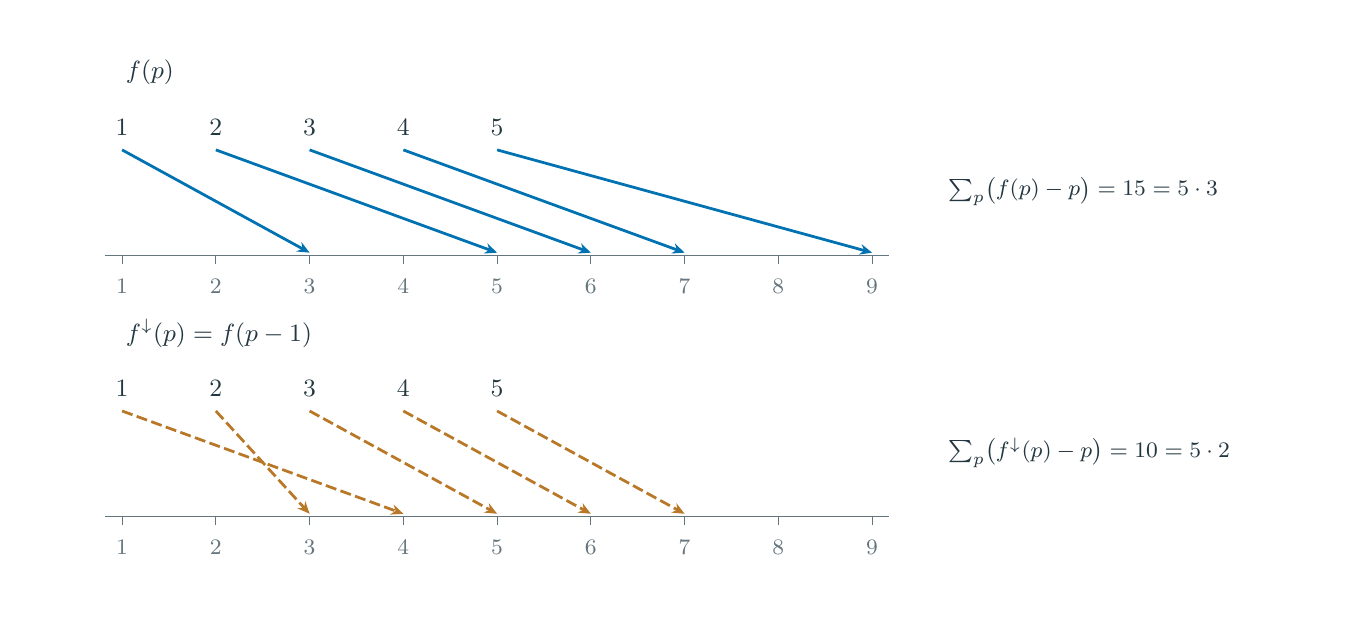
\begin{tikzpicture}[x=1bp,y=1bp]
\useasboundingbox (0,0) rectangle (468.000,204.000); %@ shift canvas w=468.000 h=204.000
\node[labm] at (34.000,168.000) {$1$}; %@ shift f top p=1 x=34.000
\node[labm] at (67.750,168.000) {$2$}; %@ shift f top p=2 x=67.750
\node[labm] at (101.500,168.000) {$3$}; %@ shift f top p=3 x=101.500
\node[labm] at (135.250,168.000) {$4$}; %@ shift f top p=4 x=135.250
\node[labm] at (169.000,168.000) {$5$}; %@ shift f top p=5 x=169.000
\draw[muted, line width=0.4pt] (28.000,122.000) -- (310.000,122.000);
\draw[muted, line width=0.4pt] (34.000,122.000) -- (34.000,119.000);
\node[idx] at (34.000,111.000) {$1$}; %@ shift f tick v=1 x=34.000
\draw[muted, line width=0.4pt] (67.750,122.000) -- (67.750,119.000);
\node[idx] at (67.750,111.000) {$2$}; %@ shift f tick v=2 x=67.750
\draw[muted, line width=0.4pt] (101.500,122.000) -- (101.500,119.000);
\node[idx] at (101.500,111.000) {$3$}; %@ shift f tick v=3 x=101.500
\draw[muted, line width=0.4pt] (135.250,122.000) -- (135.250,119.000);
\node[idx] at (135.250,111.000) {$4$}; %@ shift f tick v=4 x=135.250
\draw[muted, line width=0.4pt] (169.000,122.000) -- (169.000,119.000);
\node[idx] at (169.000,111.000) {$5$}; %@ shift f tick v=5 x=169.000
\draw[muted, line width=0.4pt] (202.750,122.000) -- (202.750,119.000);
\node[idx] at (202.750,111.000) {$6$}; %@ shift f tick v=6 x=202.750
\draw[muted, line width=0.4pt] (236.500,122.000) -- (236.500,119.000);
\node[idx] at (236.500,111.000) {$7$}; %@ shift f tick v=7 x=236.500
\draw[muted, line width=0.4pt] (270.250,122.000) -- (270.250,119.000);
\node[idx] at (270.250,111.000) {$8$}; %@ shift f tick v=8 x=270.250
\draw[muted, line width=0.4pt] (304.000,122.000) -- (304.000,119.000);
\node[idx] at (304.000,111.000) {$9$}; %@ shift f tick v=9 x=304.000
\draw[arrP] (34.000,160.000) -- (101.500,123.000); %@ shift f arrow p=1 to=3 x0=34.000 x1=101.500
\draw[arrP] (67.750,160.000) -- (169.000,123.000); %@ shift f arrow p=2 to=5 x0=67.750 x1=169.000
\draw[arrP] (101.500,160.000) -- (202.750,123.000); %@ shift f arrow p=3 to=6 x0=101.500 x1=202.750
\draw[arrP] (135.250,160.000) -- (236.500,123.000); %@ shift f arrow p=4 to=7 x0=135.250 x1=236.500
\draw[arrP] (169.000,160.000) -- (304.000,123.000); %@ shift f arrow p=5 to=9 x0=169.000 x1=304.000
\node[labm,anchor=west] at (34.000,188.000) {$f(p)$};
\node[lab,anchor=west] at (330.000,145.000) {$\sum_p\bigl(f(p)-p\bigr)=15=5\cdot3$};
\node[labm] at (34.000,74.000) {$1$}; %@ shift g top p=1 x=34.000
\node[labm] at (67.750,74.000) {$2$}; %@ shift g top p=2 x=67.750
\node[labm] at (101.500,74.000) {$3$}; %@ shift g top p=3 x=101.500
\node[labm] at (135.250,74.000) {$4$}; %@ shift g top p=4 x=135.250
\node[labm] at (169.000,74.000) {$5$}; %@ shift g top p=5 x=169.000
\draw[muted, line width=0.4pt] (28.000,28.000) -- (310.000,28.000);
\draw[muted, line width=0.4pt] (34.000,28.000) -- (34.000,25.000);
\node[idx] at (34.000,17.000) {$1$}; %@ shift g tick v=1 x=34.000
\draw[muted, line width=0.4pt] (67.750,28.000) -- (67.750,25.000);
\node[idx] at (67.750,17.000) {$2$}; %@ shift g tick v=2 x=67.750
\draw[muted, line width=0.4pt] (101.500,28.000) -- (101.500,25.000);
\node[idx] at (101.500,17.000) {$3$}; %@ shift g tick v=3 x=101.500
\draw[muted, line width=0.4pt] (135.250,28.000) -- (135.250,25.000);
\node[idx] at (135.250,17.000) {$4$}; %@ shift g tick v=4 x=135.250
\draw[muted, line width=0.4pt] (169.000,28.000) -- (169.000,25.000);
\node[idx] at (169.000,17.000) {$5$}; %@ shift g tick v=5 x=169.000
\draw[muted, line width=0.4pt] (202.750,28.000) -- (202.750,25.000);
\node[idx] at (202.750,17.000) {$6$}; %@ shift g tick v=6 x=202.750
\draw[muted, line width=0.4pt] (236.500,28.000) -- (236.500,25.000);
\node[idx] at (236.500,17.000) {$7$}; %@ shift g tick v=7 x=236.500
\draw[muted, line width=0.4pt] (270.250,28.000) -- (270.250,25.000);
\node[idx] at (270.250,17.000) {$8$}; %@ shift g tick v=8 x=270.250
\draw[muted, line width=0.4pt] (304.000,28.000) -- (304.000,25.000);
\node[idx] at (304.000,17.000) {$9$}; %@ shift g tick v=9 x=304.000
\draw[arrQ] (34.000,66.000) -- (135.250,29.000); %@ shift g arrow p=1 to=4 x0=34.000 x1=135.250
\draw[arrQ] (67.750,66.000) -- (101.500,29.000); %@ shift g arrow p=2 to=3 x0=67.750 x1=101.500
\draw[arrQ] (101.500,66.000) -- (169.000,29.000); %@ shift g arrow p=3 to=5 x0=101.500 x1=169.000
\draw[arrQ] (135.250,66.000) -- (202.750,29.000); %@ shift g arrow p=4 to=6 x0=135.250 x1=202.750
\draw[arrQ] (169.000,66.000) -- (236.500,29.000); %@ shift g arrow p=5 to=7 x0=169.000 x1=236.500
\node[labm,anchor=west] at (34.000,94.000) {$f^{\downarrow}(p)=f(p-1)$};
\node[lab,anchor=west] at (330.000,51.000) {$\sum_p\bigl(f^{\downarrow}(p)-p\bigr)=10=5\cdot2$};
%@ shift meta n=5 rank=3 sumf=15 sumg=10
\end{tikzpicture}
\end{document}
